\chapter{Current State of Online \LaTeX Editors and the Imposed Requirements on them}
This chapter is aimed at the elicitation of the status quo of other collaborative editors and users' expectations towards them.

First and foremost other existing solutions will be reviewed and then the requirements to a online \LaTeX editor elicited. Finally the elicited requirements and research findings are analysed.

\section{Review of Existing Online \LaTeX Editors}
\label{sec:existing-solutions}
There are two existing solutions, both open source software and can be freely downloaded and installed. They target the same problem as this work, which is providing a collaborative real-time online editor for \LaTeX documents, that is as the same time suitable for self-hosting. 

The first solution, \name{FlyLatex}, is a one-man-project developed by Daniel Alabi and started in 2012, to counter the lack of collaborative real-time \LaTeX environments. It matured until mid 2013, since where there were fewer updates although the project is still being actively developed \cite{website:flylatex-commits}. 

The second solution, \name{ShareLaTex}, originated from a project called \name{ScribTex}, which was the first iteration of an online \LaTeX editor, though not a collaborative one, and published in 2008. \name{ShareLaTex} is the redevelopment and -implementation of that basic concept \cite{website:scribtex} \cite{website:sharelatex}. 

Being run as a website that is free to use for up to two project members but sells subscriptions plans for projects with more members, its code base was published as open source in mid-February 2014, parallel to the draft of this work \cite{website:sharelatex-oss}. 

However, the website continues to be still run as a freemium model, meaning that the basic functionalities are free to use but more extensive features are only available when paying for them.

The architecture and implementation details of each solution will be illuminated hereafter and the findings presented in a nutshell at the end.

\subsection{FlyLatex}
\label{subsec:flylatex}
FlyLatex is developed in Node.js, a lightweight, server-side platform for network applications, built on Google Chrome's JavaScript. It is intended to help implementing data-intensive, fast, scalable applications for real-time applications with its event-driven, non-blocking I/O model \cite{website:node-js}. Moreover, the built-in asynchronous I/O library for file, socket and HTTP communication allows Node.js to act as a stand-alone web server.

Node.js was originally written and initially released on May 27th, 2009 by Ryan Lienhart Dahl. The most recent stable release, as of May 2014, is version 0.10.28.

Node.js' key feature is its performance and concurrency, which works the following way: It uses a cross-platform library that is provided by all major operating systems and abstracts system calls for asynchronous (non-blocking) input/output. Node.js is single-threaded and tells the operating system that it should be notified upon new connections. Right after that, it immediately goes to sleep and when a new connection is made, a callback is executed and the actual work then performed by Node.js.

This results in non-blocking processes, as no function in Node.js is performing input/output operations directly. That way, there are no dead-locks. In addition, it is more memory-efficient in contrast to most other programming languages concurrency models. They usually allocate memory for each new thread and connection, while in Node.js each connection allocates only a small heap.

In short, Node.js excels for thousands of concurrent connections. This is due to the fact that web servers spent a lot ot their time waiting for network or disc access, which is not CPU intensive, and Node.js performs especially well in this area. Thinking in \nameref{subsec:cloud-service-models}, it can be seen as \nameref{subsubsec:paas}, as it also provides a platform to run applications on and shares the suitablity for short-living processes.

But to return to FlyLatex: Being built on the well-illustrated Node.js and written in JavaScript, it makes use of various other technologies such as the \name{ACE Editor}, an embeddable code editor written in JavaScript, that supports syntax highlighting for over 110 languages, code completion and themes among other things \cite{website:ace-editor}. It was developed by Cloud9 for their online IDE and is published as open source on GitHub \cite{website:ace-github}.

To provide collaborative editing, FlyLatex integrates \name{ShareJS}, an operational transform (compare chapter \ref{subsubsec:operational-transform}) library for browsers and Node.js, that adds support for concurrent live editing \cite{website:sharejs}. It was written by Joseph Gentle in 2011, an ex-engineer of Google Wave, which was one of the first major products that featured collaborative editing. But it was closed by Google in 2012, due to the lack of popular demand, and is now an Incubator Project of Apache \cite{website:googlewave-status} \cite{website:apache-wave}. ShareJS is also hosted on GitHub \cite{website:sharejs-github}.

To display Portable Document Files, a viewer called \name{PDF.js} is integrated into FlyLatex. First being started by the Mozilla Foundation as an HTML5 technology experiment that explored building a precise and efficient renderer without native code assistance, it is now officially used in the Firefox browser as default plugin. 

Its major features are a search function, jump to page, zooming, fullscreen view, printing and bookmark support, save as file. Among the extensive features is also the localisation for various languages.

For data storage, FlyLatex relies on \name{MongoDB}, a document-oriented NoSQL database \cite{website:mongo-db}.

FlyLatex is hosted on GitHub \cite{website:flylatex-github}.

After an overview of the technical aspects, the functionalities and implementation will now be discussed. The following features are the ones that FlyLatex describes itself with \cite{website:flylatex-github}:

\begin{itemize}
	\item{Real-time collaboration}
	\item{Real-time status updates on priveleges of documents}
	\item{Online compilation of \LaTeX to \fileformat{PDF}}
	\item{Online \LaTeX debugging}
	\item{Manipulation of compiled \fileformat{PDF}s}
	\item{Sharing of \fileformat{PDF}s}
	\item{Option to use images or additional packages like .sty files}
\end{itemize}

Another point is missing on this list though. FlyLatex can be self-hosted on one's own Node.js server and only requires some configuration for the connection to a running MongoDB instance. This is of major importance, as one must not hand over control of sensitive data and confidential documents to other cloud providers. At the same time, information security is also maximised.

After deploying FlyLatex on Node.js and accessing the webpage in the browser, the landing page shows a login as well as the possibility to sign-up for the service. On successful login, the main page compromises of a simple document management and very basic message center where notifications of changes in documents can be seen. The exisiting documents are listed with their rights (read/write) and can be deleted or shared. New documents can be created as well. 

When sharing documents, the field uses auto-complete on the exisiting users, making it easier to find each individual person. This person then receives a notification, accessible in the message center, and the user is able to either accept or decline the access to the document.

But the core part of FlyLatex is the document editing. The editor comes with syntax highlighting and is displayed full-page. If users edit the document collaboratively, text changes are immediately applied and displayed in other users' browsers that are also working on this document, meaning there is hardly any delay. Although changes are auto-saved they are not persisted in the database, effectively resulting in loss of data when internal server errors occur or it is shutdown, it was just written to volatile memory. Changes are only persisted when explicitly clicking the document's save button.

\pagebreak

To be able to compile documents, the \fileformat{PDF} view must be activated. It provides a button to compile the document, download the \fileformat{PDF} and view the compilation log. The latter is displayed as a small overlay and can be browsed by going back and forth to each log extract. The result of the compilation, the successfully created \fileformat{PDF}, is shown in a preview right next to the editor.

\begin{figure}[H]
	\centering
		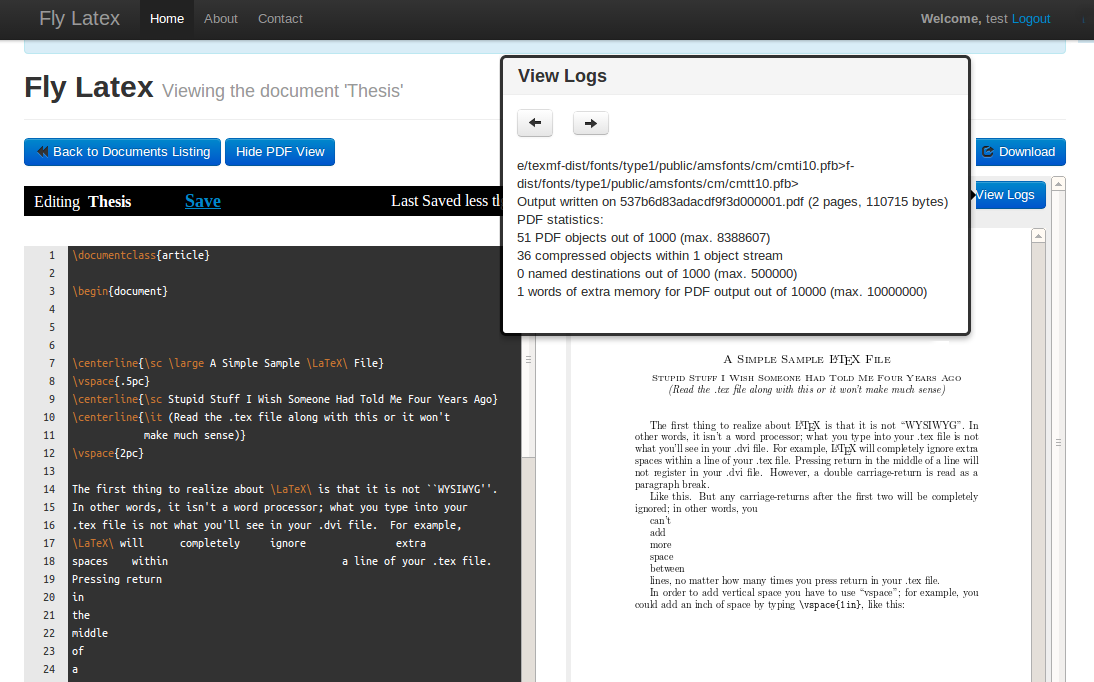
\includegraphics[width=\textwidth]{images/flylatex.png}
	\caption{FlyLatex' document editing and compilation view}
\end{figure}

If there are errors during the compilation, a notification is displayed and the log can be consulted to figure out the cause. When a document was not compiled for the first time, the last successfully compiled \fileformat{PDF} is still shown and the preview not updated.

The actual compilation is achieved by calling the console to execute the transformation of the \LaTeX document. That is why FlyLatex is expecting PDFLatex to be installed, as it is the utilised engine and hard-wired in the source code:

\begin{lstlisting}[language=JavaScript, frame=none, numbers=none, caption=Latex Compilation in FlyLatex]
exec("pdflatex -interaction=nonstopmode "+ inputPath +" > /dev/null 2>&1", 
afterCompile);
\end{lstlisting}

The \parameter{nonstopmode} specifies that the compilation will not be stopped by PDFLatex upon errors, while \parametertype{/dev/null 2>\&1} is redirecting the outputs of the console, resulting in all standard output to be repressed (signifies the compilation log) and only errors being displayed on the console. 

Finally, \parameter{afterCompile} is the name of the callback function that will be executed after successful execution of the command. The actual source code of it will not be listed, but this function reads in the \fileformat{PDF} file and makes it accessible under a unique Uniform Resource Identifier (\abk{URI}{Uniform Resource Identifier}), then reads the log as well and sends both to its own REST services. Finally, it presents the log and file to the user by showing both on the webpage.

Analysing all these information, there are several downsides to this approach:

The handling of documents is rather complicated. To change between documents, one has to go back to the main page and then select a different document to open it. 

A document is a stand-alone file, there is no possibility to structure it by seperating it into more \LaTeX files or include others. That way, bibliography management is not supported as well. 

The log is only accessible in a small overlay dialog and when trying to skip to the end, the next page button must be clicked several times. 

That shared documents have first be accepted or declined in the somewhat hidden message center also adds to the perception of a lacking user experience.

The parallel view of the document and the compiled \fileformat{PDF} is a good approach, but missing controls for zoom. Therefore a detailed examination of the output is not possible for the user, who is left with a rather vague impression about the rightfulness of the created \fileformat{PDF} file.

In conclusion, the bare collaborative document editing and document sharing is working excellent, but advanced functions such as multi-file documents, import, bibliography management and extensive \LaTeX support and tools are missing, preventing a pleasent user experience.

\subsection{ShareLaTex}
\label{subsec:sharelatex}
First and foremost, ShareLaTex cannot be equivalently compared to FlyLatex, as the former is the result of a capital-backed, longstanding project with full-time commitment of its developers. So thinking of ShareLaTeX, the sale of subscriptions makes it actually rather a business model than an open-source project \cite{website:sharelatex-team} \cite{website:sharelatex-subscriptions}. The latter is especially true as FlyLatex used to be the solely available open source online editor, with ShareLaTex being freely available only since shortly, February 2014.

The decision to go open source is justified by the developers in the following way \cite{website:sharelatex-oss}:

\begin{quotation}
As a small team, we're constantly receiving feature requests that we'd love to implement but don't have the time. We've also had a lot of offers from willing volunteers who we've had to turn away because we didn't have a framework for people to contribute. I hope that by open-sourcing ShareLaTeX we can empower our brilliant community to help improve ShareLaTeX in the ways that you want, without having to wait for the two of us to work down our todo list. \\

A lot of people have asked to host ShareLaTeX internally due to company guidelines or data privacy concerns. We don't have the resources to support licensed installs at the moment, but we also hate having to say no. With an open-source version of ShareLaTeX, now anyone who wants to run it locally can.
\end{quotation}

ShareLaTex is hosted on GitHub and consists of several subprojects and services: For the web interface, application of updates on documents, \name{Common LaTeX Service Interface} (\abk{CLSI}{Common LaTeX Service Interface}) for the compilation of \LaTeX documents, \abk{CRUD}{Create, Read, Update and Delete} operations (create, read, update, delete) operations and tracking and storing updates for documents \cite{website:sharelatex-github}.

It mostly relies on the same established technologies as FlyLatex (compare chapter \ref{subsec:flylatex}), such as Node.js, MongoDB, AceEdtior and PDF.js. 

Having said this, it makes use of one additional technology, \name{Redis}, a key-value-store used as data structure server. It is used to perform atomic operations on various data types such as Strings, Hashes, Lists, Sets and Sorted Sets, which are kept as in-memory datasets. Such operations would for instance be: appending to a String, pushing to a List, computing Set intersection, union, difference and so on \cite{website:redis}.

Before running ShareLaTex on Node.js, it must be assured that the Redis and MongoDB services are running, a suitable \LaTeX environment is installed and also a specific version of the \name{latexmk} package.

The \name{latexmk} package can be used in two ways. On the one hand, to detect the correct order and amount of times to compile a document. For example when there is a bibliography and a nomenclature, the execution order would be \method{pdflatex bibtex pdflatex makeindex pdflatex} as the document has to be first compiled. Then the citation references would be set by \method{bibtex}, added to the document in the second compilation step and finally the same would apply for the nomenclature with the last two commands.

On the other hand, \name{latexmk} is even more powerful as it can be used to watch \TeX files for changes and run the necessary commands to re-compile the \fileformat{PDF} automatically.

ShareLaTex comes with several matured functionalities. In addition to the basic CRUD operations, it also supports the inclusion of other files or  even structuring a project with subdirectories. There are various ways to share documents, either with specific users - for which their e-mail has to be entered - or by URI. If the latter is chosen, projects can be made either publicly readable or editable, providing also access to users outside of the platform. Besides, exisiting projects can be download and new projects imported as ZIP file.

There are also specific project settings, as for the spellchecking language of documents, setting the main document and which compiler (PDFLaTeX, LuaTeX, XeLaTeX) to use, whereas some features are exclusively available to the website. Such as the newly introducted integration of DropBox, templates, the help and a \LaTeX tutorial.

\pagebreak

But the centrepiece is the document editing view, which also combines the preview of the compilated \fileformat{PDF} and raw compilation log. There are, from left to right, a foldout sidebar with icons for the code, history, sharing and settings of the document, the project file tree where files can be added, renamed, deleted, the editor containing the document's \LaTeX code and the mentioned preview for \fileformat{PDF} and log.

\begin{figure}[h!]
	\centering
		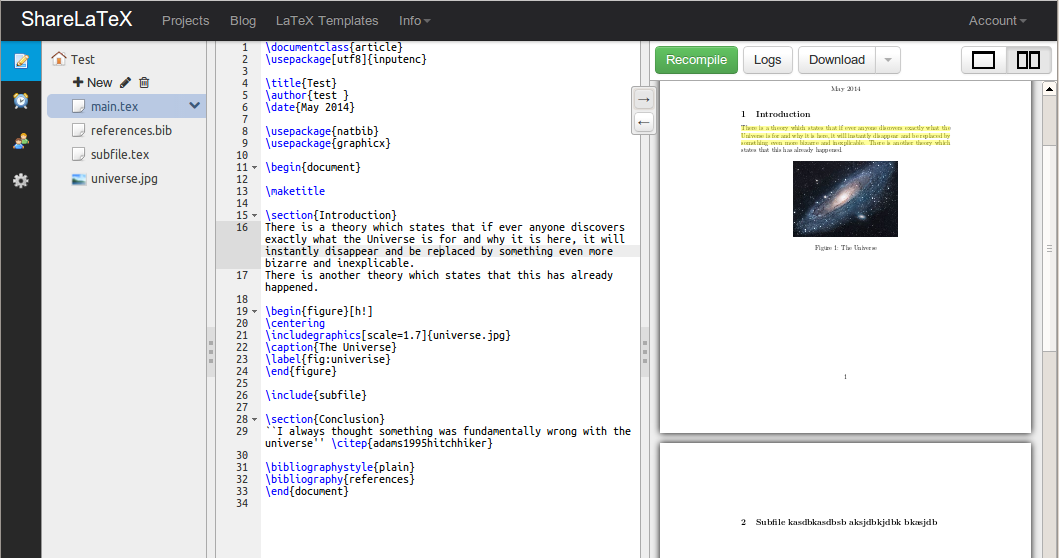
\includegraphics[width=\textwidth]{images/sharelatex-editing.png}
	\caption{ShareLaTex' document editing and compilation view}
	\label{sharelatex-editing-view}
\end{figure}

As ShareLaTex makes use of the same most commonly used and proven library \name{ShareJS} to enable collaborative editing, changes in documents can be seen instantly in other browsers. If a document is edited by several individuals, each user's current cursor position is shown in a different colour to make it clearly recognisable on which part of the document he is presently working. Changes are instantaneously persisted in the database, code completion is provided by the editor.

When there are errors during compilation, they are automatically extracted from the log and presented in summary, with description and cause. As a matter of course the raw log output can be viewed was well.

\begin{figure}[h!]
	\centering
		
\includegraphics[width=0.66\textwidth]{images/sharelatex-error.png}
	\caption{ShareLaTex' summarises errors with description and cause}
\end{figure}

Document compilation is quick and the preview has, unlike FlyLatex, also zoom buttons to take a closer look at the \fileformat{PDF}. The split view of document code and \fileformat{PDF} can be switched to a single view, where either the editor or preview is shown on the entire screen. The sidebar and project file tree remain displayed though.

A rather sophisticated feature is the possibility to click either on parts of the document to see the corresponding code passages or the other way around, where for any code passage the according output in the \fileformat{PDF} is highlighted in a pale yellow tone (as can be seen on the upper right in figure \ref{sharelatex-editing-view}).

If document changes shall be tracked, there is a history where changes are depicted in a timeline. Each modification is shown with time and the user causing it on a sidebar on the right. When clicking on one of these entries, the document's version as of that point in time is displayed in the editor. User's changes are represented in a different color, actually showing a diff of the document. This is quite helpful to spot changes immediately. With this functionality comes also the option to restore the document back to its state of that given point. All in all, this is equivalent to a basic revision control system.

\begin{figure}[h!]
	\centering
		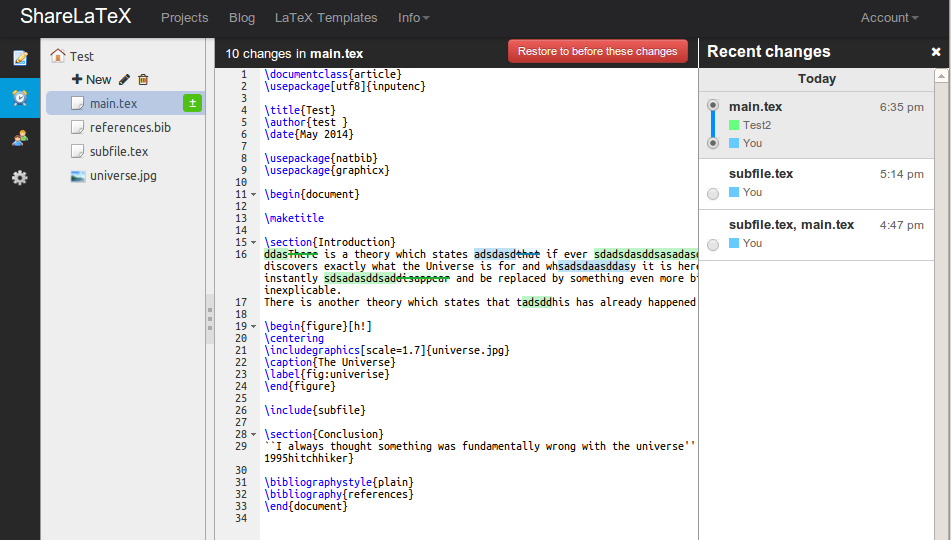
\includegraphics[width=\textwidth]{images/sharelatex-history.png}
	\caption{ShareLaTex' document history view}
\end{figure}

Finally, there are even user settings where the preferred editor theme, font size, key binding can be adjusted, autocompletion switched on or off as well as the user's data and password reset.

The implementation of the compilation is quite similiar to FlyLateX', the process is spawned directly from the command line. Because of the more complex architecture and distributed code base of ShareLaTeX, the actual source code will only be shown in excerpts and for the compilation engine \name{PDFLaTeX}.

\pagebreak

\begin{lstlisting}[language=JavaScript, frame=none, numbers=none, caption=Latex Compilation in ShareLaTeX]
_latexmkBaseCommand: ["latexmk", "-cd", "-f", "-jobname=output", "-auxdir=$COMPILE_DIR", "-outdir=$COMPILE_DIR"]:
return LatexRunner._latexmkBaseCommand.concat(["-pdf", "-e", "$pdflatex='pdflatex -synctex=1 -interaction=batchmode %O %S'", Path.join("$COMPILE_DIR", mainFile)]);
[...]
}).call(this);
\end{lstlisting}

Again, the \parameter{nonstopmode} is used to make the compilation not hold upon errors, as well as a callback function is executed on completion. The major differences are the use of \name{latexmk} (as mentioned earlier a package for automatic document (re-)compilation) and the parametrisation of the compilation engine (here \name{PDFLaTeX}).

Evaluating ShareLaTex' implementation and features, the collaborative nature of its service is ubiquitously noticeable in several functionalities such as the history. It is one of ShareLaTex' strong points, together with document editing, hierarchical structuring, sharing and performance. But there are also weaknesses regarding the support of bibliography and \LaTeX functions, although the latter is partly implemented by the editor's code completion. Nevertheless, ShareLaTex provides a good user experience with all necessary basic functions and even rather useful additional features. 

\subsection{Findings}
Analysing the findings for both existing solutions, \nameref{subsec:flylatex} and \nameref{subsec:sharelatex}, there are several similiarities because of their use of the almost same technologies. 

Both are based on Node.js, which performs and scales very well as lightweight, server-side platform for network applications. It is well-suited as the creation of diffs and application of patches on texts is not very CPU intensive, although the \LaTeX to \fileformat{PDF} compilation is, to a certain amount.

They also share their approach of document compilation: First the command is executed on the console and then a callback function used to process the output further.

Collaborative editing works like a charm on ShareLaTeX and FlyLatex by using ShareJS, there are no noticeable delays and document changes are always applied in the correct way.

Regarding all functions beyond the basics, ShareLaTeX excels FlyLatex in the user experience and the provisioning of useful tools by far. This is obviously the result of long dedication to the project and capital-backed development, while FlyLatex must be seen as what it is: a spare time project of a single developer.

Having been closed-source for most of it's development lifespan, ShareLaTex was a late competitor to the race but is now the leading open-source \LaTeX editor for people or organisations who are dedicated to keep their private data in their own hands. 

However, as can be seen in the next section, neither of the solutions fulfills all requirements for such a collaborative online \LaTeX editor. And above all else, they would also not satisfy the need for an application that utilises the exisiting infrastucture (compare chapter \ref{sec:scope-and-aim} and chapter \ref{sec:approach-and-decision}) of the Institute of Telematics. 

\section{Technical Constraints and Software Requirements}
For the development of a cloud-based \LaTeX editor, there are some technical constraints, predefined by the Institute of Telematics' computing resources, as well as software requirements - be it implicit requirements declared in advance to this work or the one's defined in the preliminary stages by inquiry of the future users.

In the following sections, both contraints and requirements are evaluated to work out the implications for the outcome of this work. First off, the computing resources, topology and technology of the Institute of Telematics' Cloud Computing Lab are treated, then followed by the elaboration of functional and implicit requirements in the next section.

\subsection{Technical Constraints}
\label{subsec:technical-constraints}
The technical contraints consist of various factors such as computing resources, so existing hardware, its arrangement, network topology and ultimately its configuration, especially the systems' architectures, operating systems and middlewares.

These are the variables that will be looked at throughout the following subsections, although it must be noted that only the parts closely related to this work will be reviewed in detail.

\subsubsection{Computing Resources}
\label{subsubsec:computing-resources}
The Cloud Lab's infrastructure is made up of a heterogenous array of computers and servers, ranging from older AMD64 or Intel Core 2 Duo with 2GB of RAM to the new generation of Intel Core i7 with 8GB RAM and therefore reflecting the variances in Cloud Computing systems in a realistic way. 

The topology can be roughly divided into four parts: There are the firewall and the \abk{DNS}{Domain Name System} servers, ensuring network communication and protection of the affiliated systems and then workstations for employees and students. Its most central part though are the different clouds to test a diversity of different infrastructures. 

For such purposes, there are two main clouds, one is based on OpenStack, the other one on Eucalyptus, and then there are two test clouds where more recent versions or new developments in the Cloud Computing landscape can be installed and examined \cite{website:openstack} \cite{website:eucalyptus}. \\
All the mentioned components of the lab can be seen in the network topology below.

\begin{figure}[H]
	\centering
		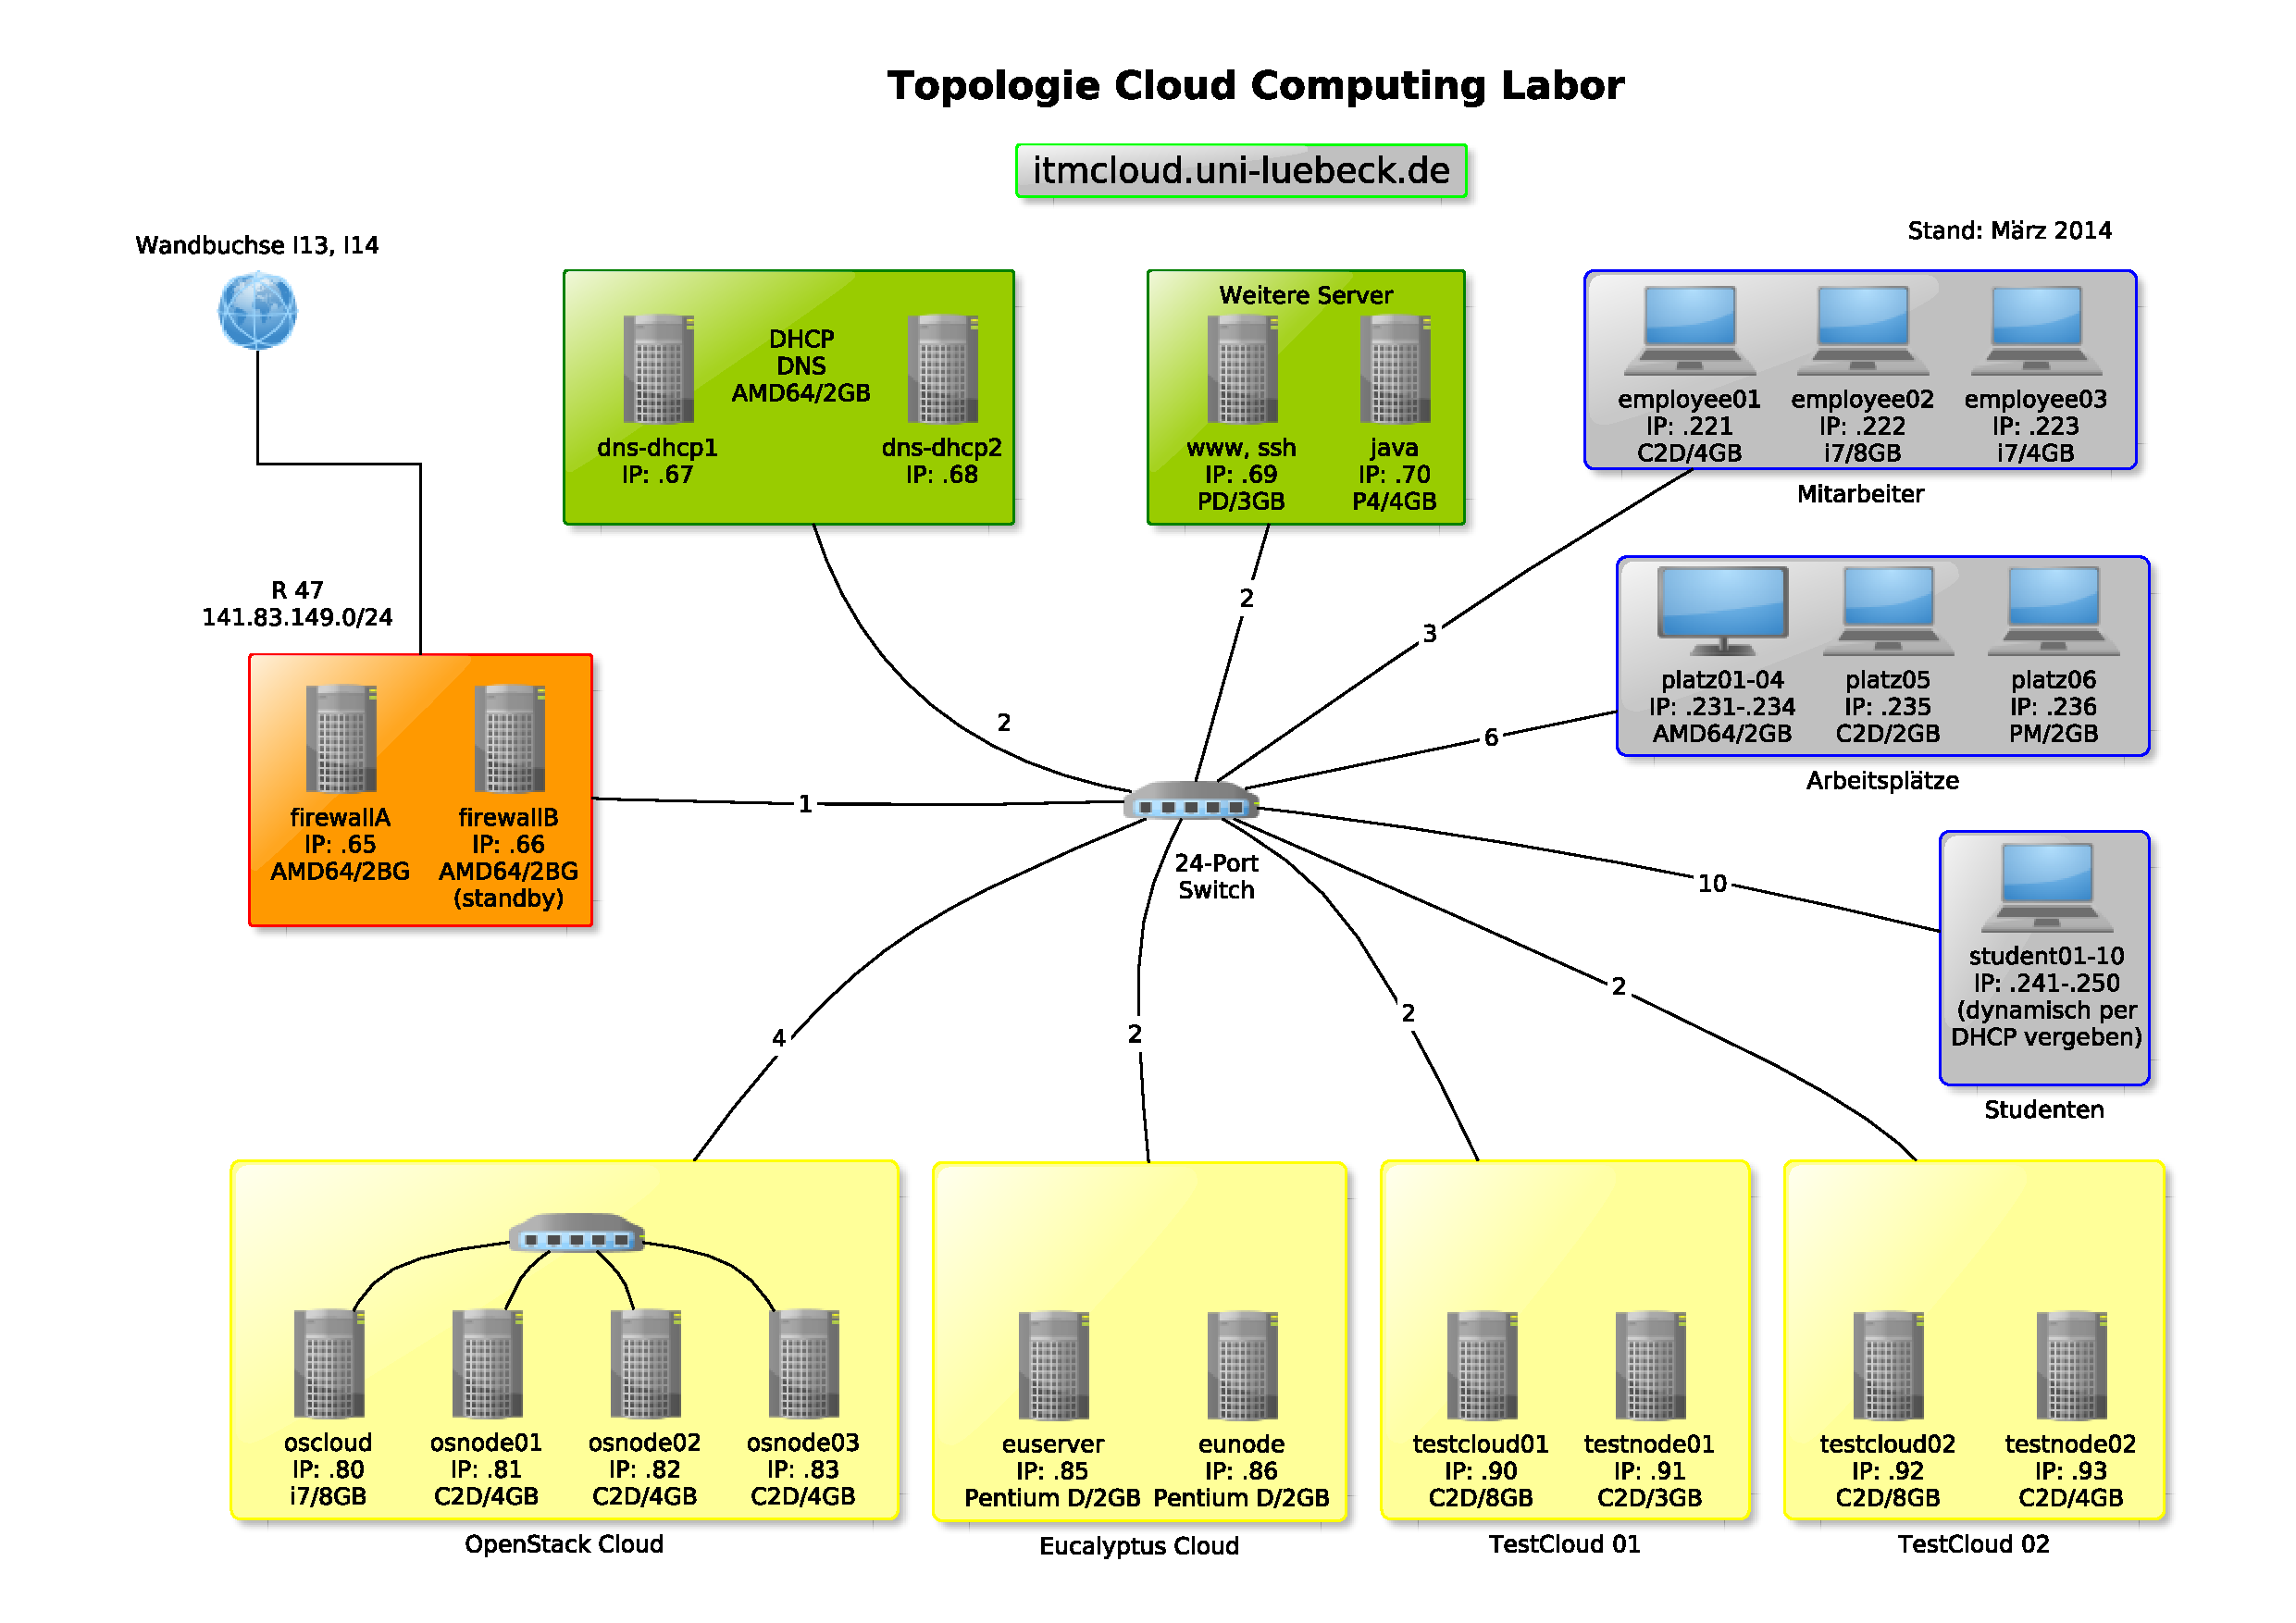
\includegraphics[width=\textwidth]{images/itm-topology.pdf}
	\caption{The topology of the University of L\"ubeck's Institute of Telematics' Cloud Computing Lab}
\end{figure}

Subsequently, only the OpenStack cloud and its characteristics will be regarded as it is the most suitable cloud, which will be explained alongside the depiction of its architecture. For further information on the comparision of different open source Clouds compare the preceding bachelor thesis of Thomas Moritz \cite{thomas2013cloud}.

It should be pointed out that details on the actual configuration are omitted, as this work takes a fully configured and working system as starting point, which is the case with the ITM Cloud Computing Lab.

\subsubsection{OpenStack}
\label{subsubsec:openstack}

OpenStack began in 2010 as mutual project of the NASA and Rackspace Hosting and is now established as non-profit foundation, with many major tech companies like Microsoft, IBM, Oracle or Red Hat being contributers and members of the project. It consists of the components:

\begin{itemize}
	\item{\name{Horizon} serves as a dashboard, a web front-end to manage and control the Cloud and its services}
	\item{\name{Nova} is executing the virtual machines}
	\item{\name{Swift} persists objects and is a highly scalable system where user and instances can store data}
	\item{\name{Glance} manages images and snapshots of virtual machines}
	\item{\name{Keystone} is used for authentification and rights management}
	\item{\name{Quantum} controls the routing and network}
	\item{\name{Cinder} is a block storage that provides logic volumes}
\end{itemize}

The interdependency and relation between these components can be seen in the following graph.

\begin{figure}[h!]
	\centering
		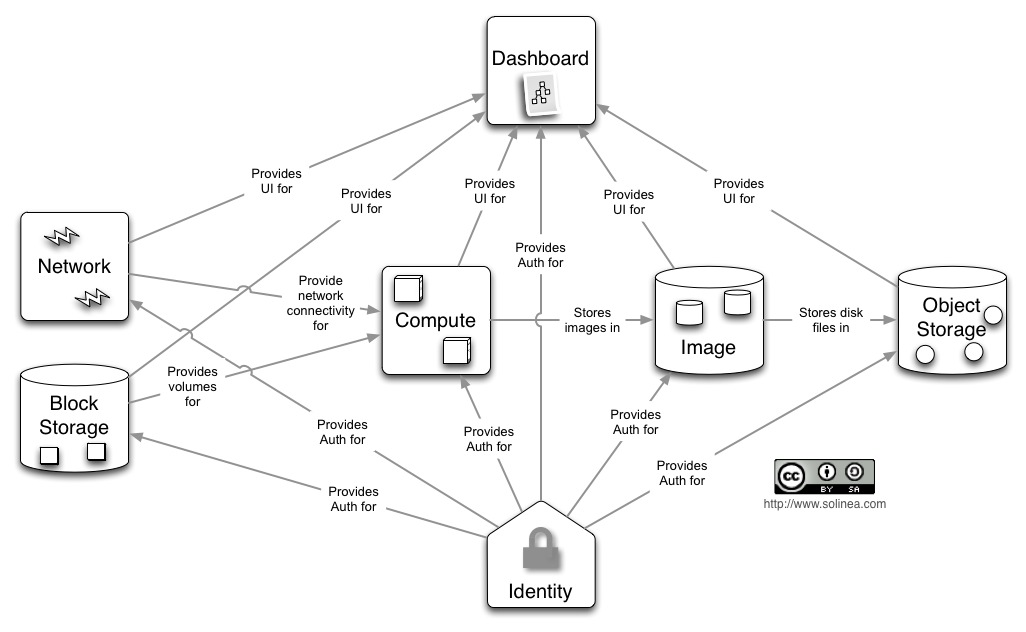
\includegraphics[width=0.9\textwidth]{images/openstack-architecture.png}
	\caption{The architecture and component relations of OpenStack \cite{website:wikimedia-openstack-conceptual}}
\end{figure}

As this is a bit abstract to grasp, there is also a more simplyfied version showing how {OpenStack} provides the basis to build applications on top of it.

\begin{figure}[H]
	\centering
		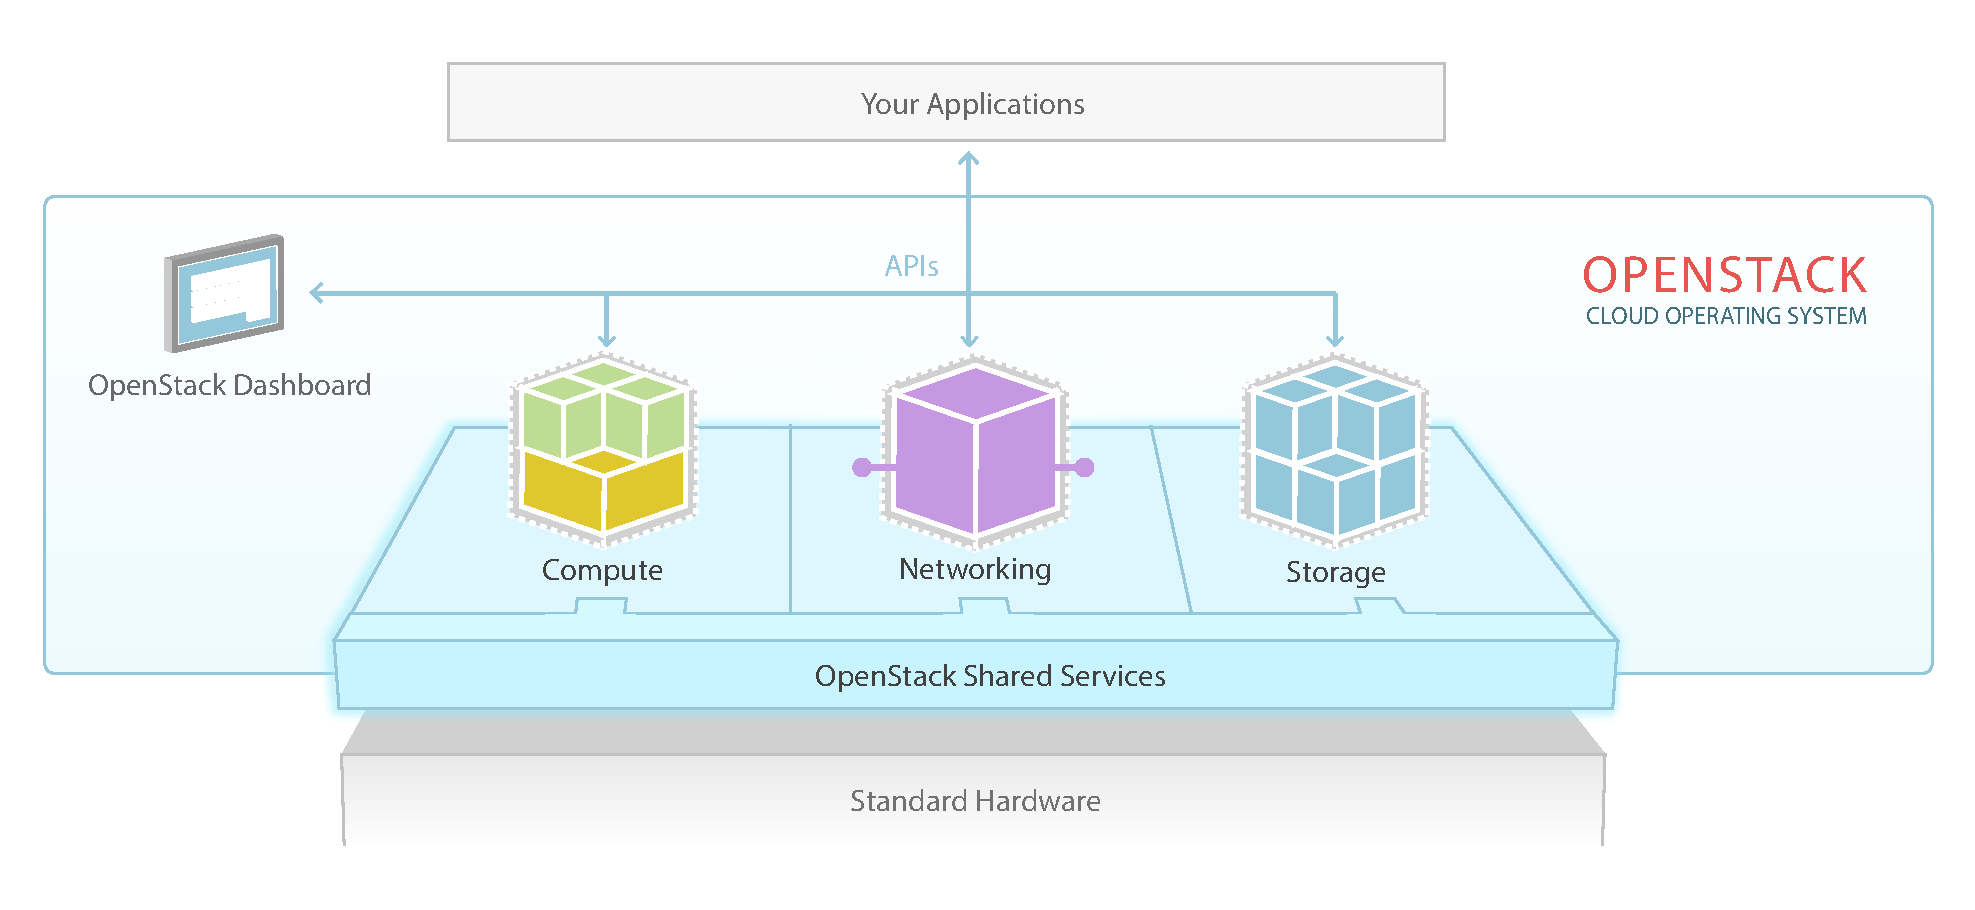
\includegraphics[width=\textwidth]{images/openstack-software-diagram.pdf}
	\caption{Simplyfied OpenStack software diagram \cite{website:openstack-sw-diagram}}
\end{figure}

OpenStack is acting as IaaS and implements simple and massively scaleable cloud services that can be used to provide public or private clouds (compare \nameref{subsec:cloud-deployment-models}, chapter \ref{subsec:cloud-deployment-models}). As can be seen from the graphics, such services include the creation of pools for compute, storage and network resources, which can then be used to virtualise one's server hardware. This happens in a way, that the virtualisation layer abstracts the resource management and specifics of the existing hardware, making both of no concern to the consumer.

The advantages are apparent: While OpenStack is simple to integrate with any hardware, easy to manage and monitor, secure and an industry-wide standard, the systems build on OpenStack are also very elastic, highly available and realiable.

\subsection{Software Requirements}
\label{subsec:software-requirements}
In a software project, requirements engineering, namely the formulation, collection, documentation and maintenance of software requirements, is certainly the most vital part, being not much different for this work. 

There are two main stakeholders, first the users and secondly the operators. While most requirements originate from the users, there were also some requirements couched by the operators. This is potentially leading to conflicts of interest and will be described later, but first all requirements are listed. They are documented as they arised, starting with implicit requirements and followed by the functional ones.

\subsubsection{Implicit Requirements}
\label{subsubsec:implicit-requirements}
There are a number of implicit requirements that were already partially discussed in section \ref{sec:scope-and-aim}, \nameref{sec:scope-and-aim}. These are basic conditions that were defined prior to this work with the supervisor.

To begin with, the application is supposed to run as SaaS. Secondly, it is vital that different users can not only edit documents together but also simultaneously, making the collaborative aspect of the application its most important feature. 

When desired, the current \TeX document has to be compiled and the result shown to the user. Document changes shall be backed by the usage of a version control system that ensures all document revisions are stored and can be restored.

Lastly, access should solely be granted to users of the Institute of Telematics, who will use their exisiting \name{Lightweight Directory Access Protocol} (\abk{LDAP}{Lightweight Directory Access Protocol}) accounts for authentification.

\subsubsection{Functional Requirements}
\label{subsubsec:functional-requirements}
While all these implicit requirements are primarily shaping the architecture of the system, the actual features are defined by functional requirements which are compiled of the later users' requests and needs. 
 
To gather these data, a questionnaire with a list of possible features was prepared. Each functionality could be ranked on a scale from 1, \textit{not so important}, to 10, \textit{very important} and additional remarks or feature requests be made. 

There was a total of 21 questions and a response from 18 individuals, with the highest rating being a 8.7 and the lowest a 4.2. The arithmetic mean was 6.8 and the median 7.0. 

Based on their values, these functionalities were prioritised and divided into three majors groups: \textit{high priority}, \textit{medium priority} and \textit{low priority}. The size of each group was arranged after the arithmetic mean, respectively median, so that the group of highest prioritisation has five functionalities and a arithmetic mean and median of 8.1.

\begin{table}[H]
	\begin{center}
		\footnotesize
		\setlength\extrarowheight{5pt}
		\rowcolors{1}{}{lightgray}
		\begin{tabular}{ p{11cm} cp{1.5cm} }
		  	\textbf{Functionality} 	  														& \textbf{Rating} \\
			\hline
			Undo/Redo of edits																& 8.7 \\
			Support of bibliography/BibTeX management										& 8.3 \\
			Viewable log of the compilation													& 8.3 \\
			Automatic background save while editing (e.g. every five minutes)				& 8.1 \\
			Tabs for multiple opened documents and parallel editing							& 8.0 \\
		\end{tabular}
		\caption{Functionalities with high priority}
		\label{tab:high-priority}
	\end{center}
\end{table}

While the group with medium priority has the same arithmetic mean and median as the overall results of 6.8 and 7.0, consisting of six priorities.

\begin{table}[H]
	\begin{center}
		\footnotesize
		\setlength\extrarowheight{5pt}
		\rowcolors{1}{}{lightgray}
		\begin{tabular}{ p{11cm} cp{1.5cm} }
		  	\textbf{Functionality} 	  														& \textbf{Rating} \\
			\hline
			Download of single files/the whole project										& 7.8 \\
			Full-text search over all documents												& 7.6 \\
			Import function for existing \LaTeX projects									& 7.3 \\
			Code completion similiar to an IDE												& 7.1 \\
			Notifications on changes made by other users or their activities				& 7.1 \\
			Download of single files/the whole project										& 7.0 \\
		\end{tabular}
		\caption{Functionalities with medium priority}
		\label{tab:medium-priority}
	\end{center}
\end{table}

All other proposed functionalities form the group of lowest prioritisation, including ten features. This group has an arithmetic mean of 5.5 and median of 5.7.

\begin{table}[H]
	\begin{center}
		\footnotesize
		\setlength\extrarowheight{5pt}
		\rowcolors{1}{}{lightgray}
		\begin{tabular}{ p{11cm} cp{1.5cm} }
		  	\textbf{Functionality} 	  														& \textbf{Rating} \\
			\hline
			Rights management for documents (not accessible for others, share with user)	& 6.5 \\
			Preview of the document as parallel view of \LaTeX and \fileformat{PDF}			& 6.5 \\
			Existing logins can be used (authentification by LDAP)							& 6.1 \\
			Toolbar for the most common commands (bold text, section, figure et cetera)		& 6.1 \\
 			Capability to print documents													& 6.1 \\
			Personalised settings of editor appearance (font size, theme and so on)			& 6.0 \\
			Collection of formulas, extended commands, symbol tables						& 5.7 \\
			Bookmarks/markers can be set in documents				 						& 5.3 \\
			\LaTeX templates to follow the ITM conventions									& 5.0 \\
			Syntax highlighting for other languages except \LaTeX							& 4.2 \\
		\end{tabular}
		\caption{Functionalities with low priority}
		\label{tab:low-priority}
	\end{center}
\end{table}

These functional requirements defined by the users are accompanied by the requests and needs of the other stakeholders, the operators: 

When using \LaTeX engines for the compilation of documents, they are executed via command line. Granting access for a process or application to the command line is always a security risk, so instead of direct interaction with the shell, an alternative should be achieved by all means.

\section{Analysis of the Elicited Requirements and Research Findings}
The \nameref{sec:existing-solutions} and the functional requirements (compare chapter \ref{subsec:software-requirements} et seqq) for such a  collaborative editor gave diverse insights of established systems and users' expectations towards them. 

To make these components or aspects more accessible, they are divided into different groups regarding such an editor, before contemplating their implications for the development of a collaborative online \LaTeX editor.

\begin{description}
	\item[Architecture] \hfill \\
		The editor must be developed as Software as a Service.
	\item[Editor] \hfill \\
		Collaborative, simultaneous editing is an implicit requirement and therefore a must. \\
		Undo/Redo of edits, automatic saving while editing, tabs for multiple opened documents, code completion, syntax highlighting for other languages except \LaTeX are functional requirements.
	\item[Handling of LaTeX files] \hfill \\
		Compilation of \LaTeX files and showing the output to the user is an implicit requirement and therefore a must. \\
		A viewable log of the compilation, support of a bibliography, an import function for existing \LaTeX files, download of single files/the whole project are functional requirements.
	\item[Sharing] \hfill \\
		Rights management for documents and notifications on changes made by other users are functional requirements.
	\item[Personalisation] \hfill \\
		Authentification by existing LDAP accounts is an implicit requirement and therefore a must. \\
		Personalised settings of editor appearance (font size, theme and so on) and \LaTeX \linebreak templates to follow the ITM conventions are functional requirements.
	\item[User Experience] \hfill \\
		Tracking document changes with a version control system is an implicit requirement and therefore a must. \\
		A full-text search over all documents, preview of the document as parallel view of \linebreak \LaTeX and \fileformat{PDF}, capability to print documents, toolbar for the most common commands, collection of formulas and extended commands, bookmarks in documents are functional requirements.
\end{description}

To develop the application as \nameref{subsubsec:saas} limits the architectural choices, as does the fact that \nameref{subsubsec:openstack} is used in the ITM Cloud Computing Lab. To mention it again, both existing solutions are developed on \name{Node.js}.

In addition to it, \nameref{subsec:sharelatex} and \nameref{subsec:flylatex} equal themselves in two other integral parts. For the editor, \name{ACE Editor} is used, to compute and apply the right \nameref{subsubsec:operational-transform} steps, \name{ShareJS}. Both the editor and the collaboration library are too complex to develop them from scratch, so it is inevitable to make use of frameworks or libraries or embed existing applications.

The handling of \LaTeX files must be accomplished in a transparent way that seems intuitive to the user. It must be possible for him to work in an accustomed manner, for instance including other \LaTeX files, images and bibliography, while also providing functionalities to import data to and export data from the application.

As major enabler of collaboration, sharing functionality bases on document rights as well as the detailed illustration of changes performed on the document.

Personalisation can only occur when user accounts are integrated into the application and it encompasses of settings for editor theme, font size and so forth, but also document templates.

The analysing of \nameref{subsec:sharelatex} and \nameref{subsec:flylatex} emphasised the importance of functionalities and user interfaces that assist users and encourage them to take advantage of the broad range of auxiliary tools that are being provided. It must be said that both were lacking in this area, \nameref{subsec:flylatex} even more than \nameref{subsec:sharelatex}, but also the latter did not provide \LaTeX specific toolbars and menus.
